\section{Question 4}

    The given values are the following: $t_A = t_B = 5, t_C = 7, t_D = 15, t_E = 8, t_F = 10,t_G = 15, t_H = 14, t_I = 5$. Below is a tree-based calulation of WCET bound:

    \begin{figure}[H]
        \centering
        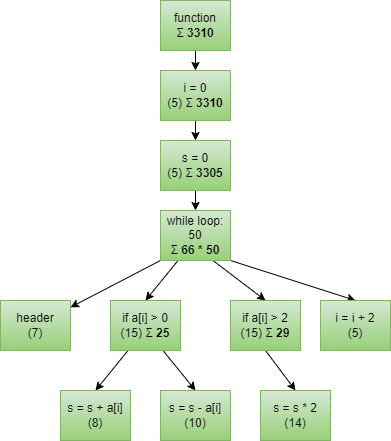
\includegraphics[height=350px]{images/Ass3Q4.png}
        \caption{This is the tree-based calculation for WCET bound.}
        \label{fig:tree}
    \end{figure}
    
    In figure \ref{fig:tree} we can see that the WCET bound found using the tree-based calculation is $3310$. The sum for the loop was found by first finding the max time for each decision statement. This is done by finding the children of the \textit{if statement} with the longest execution time and sum up that time with the time of the \textit{if statement} itself. After this has been done for all decision statements the sum of the loop is found by summing up all children of the loop and multiplying it by the tight upper bound for the loop. After this is done the execution times for A and B is added to the sum to find the WCET bound. Note, the tight upper bound for the loop is set to $50$ and not $51$ since the last iteration of will not enter the loop.